\documentclass[sans]{beamer}
\usepackage[utf8]{inputenc}
\usepackage[T1]{fontenc}
\usepackage[brazilian]{babel}
\usepackage{fixltx2e}
\usepackage{graphicx,svg}
%\usepackage{subfig}
\usepackage{longtable}
%\usepackage{wrapfig}
%\usepackage{soul}
\usepackage{textcomp}
\usepackage{amsmath}
%\usepackage{mathtools}
\usepackage{marvosym}
\usepackage{wasysym}
\usepackage{latexsym}
\usepackage{amssymb}
\usepackage{multicol}
\usepackage{pifont} %,bbding}%%,dingbat} %%% ver manual de simbolos
\usepackage[final]{listings}

\usepackage{hyperref,url}
\usepackage{comment}

%%%\usepackage{scrhack}
%\usepackage{minted}
\definecolor{azulclaro}{rgb}{0.9,0.9,1}
\definecolor{mygreen}{rgb}{0,0.6,0}
\definecolor{mygray}{rgb}{0.5,0.5,0.5}
\definecolor{mymauve}{rgb}{0.58,0,0.82}

\lstdefinestyle{myPrologstyle}
{
    language=Prolog,
    basicstyle = \ttfamily\color{blue},
    moredelim = [s][\color{black}]{(}{)},
    literate =
        {:-}{{\textcolor{black}{:-}}}2
        {,}{{\textcolor{black}{,}}}1
        {.}{{\textcolor{black}{.}}}1
}

\usetheme{Boadilla}
%Global Background must be put in preamble
\usebackgroundtemplate%
{%
    
\includegraphics[width=\paperwidth,height=\paperheight]{fundoprog2.jpeg}%
}



\graphicspath{{/home/pv/Dropbox/Picat-Apresentação/}{figures/}}

\title[Tutorial de P.I.C.A.T]{Tutorial de P.I.C.A.T}
\author[Paulo \& Claudio]{Paulo Victor de Aguiar\\
	Claudio Cesar de Sá e Outros\\ 
	Universidade do Estado de Santa Catarina -- UDESC\\
	Departamento de Ciência da Computação -- DCC\\
	Joinville -- SC}

\lstset{
  basicstyle=\small
  }


\begin{document}



\begin{frame}[fragile]   %%%% indica que o ambiente  FRAME é frágil
\maketitle
\end{frame}

%%%%%%%%%%%%%%%%%%%%%%%%%%%%%%%%%%%%%%%%%%%%%%%%%%%%%%%%%%%%%%%%%%%%%%%%

\begin{frame}[fragile]   %%%% indica que o ambiente  FRAME é frágil
\frametitle{Indice}
\tableofcontents
\end{frame}

%%%%%%%%%%%%%%%%%%%%%%%%%%%%%%%%%%%%%%%%%%%%%%%%%%%%%%%%%%%%%%%%%%%%%%%%

\section{Introdução}
\begin{frame}[fragile]   %%%% indica que o ambiente  FRAME é frágil
\frametitle{Introdução}
\begin{block}{O que é P.I.C.A.T?}
 \begin{description}
 \item [\textit{\underline{P}attern-matching}:] Utiliza o conceito de casamento de padrão. 
  
 \item [\textit{\underline{I}ntuitive}:] O Picat oferece atribuições e laços de repetição (\textit{loops}) para a programação dos dias de hoje.
 
 \item [\textit{\underline{C}onstraints}:] Picat suporta a programação por restrições.
 
 \item [\textit{\underline{A}ctors}:] Atores são chamadas orientadas a eventos.
 
 \item [\textit{\underline{T}abling}:] É possível guardar o resultado de certas operações na memória.
 
 \end{description}
\end{block}
\end{frame}

%%%%%%%%%%%%%%%%%%%%%%%%%%%%%%%%%%%%%%%%%%%%%%%%%%%%%%%%%%%%%%%%%%%%%%%%

\begin{frame}[fragile]   %%%% indica que o ambiente  FRAME é frágil
\frametitle{Introdução}
\begin{block}{Histórico}
  O P.I.C.A.T é uma linguagem multiparadigma projetada para aplicações gerais de programação.
  Foi criada em 2013 por Neng-Fa Zhou e Jonathan Fruhman utilizando o B-Prolog como base na implementação.  
  Ambas as linguagens utilizam regras lógicas na programação, porém o P.I.C.A.T possui mais funcionalidades.
\end{block}
\end{frame}

%%%%%%%%%%%%%%%%%%%%%%%%%%%%%%%%%%%%%%%%%%%%%%%%%%%%%%%%%%%%%%%%%%%%%%%%

\begin{frame}[fragile]   %%%% indica que o ambiente  FRAME é frágil
\frametitle{Introdução}
\begin{block}{Comparação com outras linguagens}
\begin{table}[!bh]
\centering
%\caption{Comparativo entre algumas linguagens}
\label{tabela_ling_refs}
{\small
%%%\begin{tabular}{c|c|c|c|c|c|c}\hline \hline
%\begin{tabular}{C{2cm}|C{1.4cm}|C{1.4cm}|C{1.4cm}|C{1.4cm}|C{1.4cm}|C{1.4cm}}\hline \hline
\begin{tabular}{p{2cm}|p{1.45cm}|p{1.45cm}|p{1.45cm}|p{1.45cm}|p{1.45cm}}\hline \hline
      &\textbf{C}  &  \textbf{Haskell} &  \textbf{Java} &  \textbf{Prolog} &  \textbf{P.I.C.A.T}\\ \hline \hline
	    
Paradigma(s)	                        & procedu-ral                                    & funcional                               & orientado à objetos   &  lógico                                             & multi-paradigma \\
\hline 

Tipagem	        & fraca                                         & forte                                   & forte                  &  fraca                                                         & fraca \\
\hline 

Verificação de tipos	                & estático                                      & estático                                & estático                              & dinâmico                                   & dinâmico \\

\hline  
Possui segurança?	                & não                                             & sim                                      & sim                                            & sim                                          & sim\\

\hline  
Passagem de parâmetros	                &  valor & -                                       &  valor                                     &  valor & casamento \\

\hline   
Legibilidade	  & baixa   & média     & média &  média       & boa \\


\hline 
\hline
\end{tabular} 
}

\end{table}
\end{block}
\end{frame}

%%%%%%%%%%%%%%%%%%%%%%%%%%%%%%%%%%%%%%%%%%%%%%%%%%%%%%%%%%%%%%%%%%%%%%%%

\begin{frame}[fragile]   %%%% indica que o ambiente  FRAME é frágil
\frametitle{Introdução}

 \begin{figure}[!ht]
 \centering
 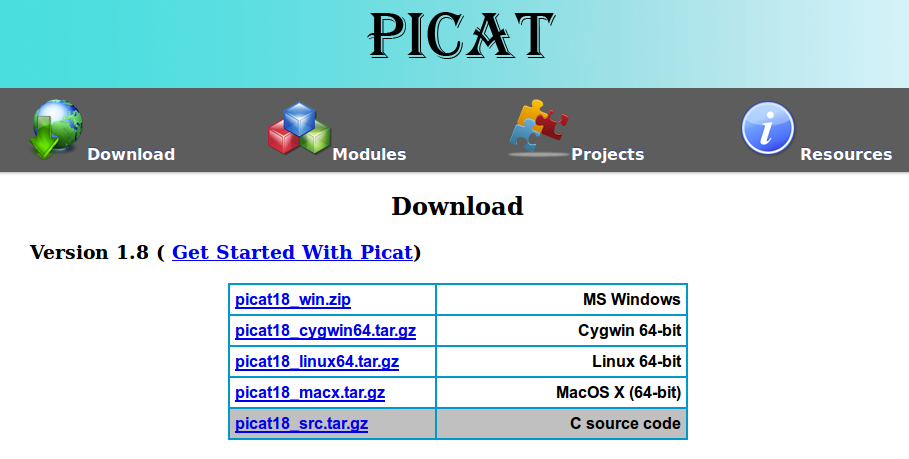
\includegraphics[width=.8\textwidth]{picatinstall.png}
 \caption{\url{http://picat-lang.org/download.html}}
 %\label{Hiera}
 \end{figure}

\end{frame}

%%%%%%%%%%%%%%%%%%%%%%%%%%%%%%%%%%%%%%%%%%%%%%%%%%%%%%%%%%%%%%%%%%%%%%%%

\section{Tipo de dados}
\begin{frame}[fragile]   %%%% indica que o ambiente  FRAME é frágil
\frametitle{Tipo de dados}

 \begin{figure}[!ht]
 \centering
 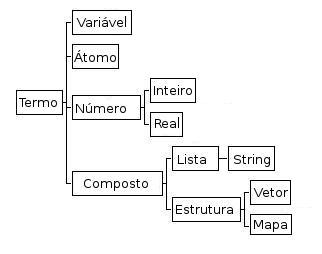
\includegraphics[width=.6\textwidth]{tipos_dados_picat_traduzido.jpg}
 \caption{Hierarquia dos Tipos de dados}
 %\label{Hiera}
 \end{figure}

\end{frame}

%%%%%%%%%%%%%%%%%%%%%%%%%%%%%%%%%%%%%%%%%%%%%%%%%%%%%%%%%%%%%%%%%%%%%%%%

\begin{frame}[fragile]   %%%% indica que o ambiente  FRAME é frágil
\frametitle{Tipo de dados}

\begin{block}{Operadores básicos}
\begin{table}[!ht]
%\caption{Tabela de Operadores}
\label{tab1}
\centering
\begin{tabular}{c|c|l}\hline \hline 
\textbf{Precedência}	&  \textbf{Símbolo} &  \textbf{Significado}\\ \hline \hline
	    
\textit{Alta}	&  \textit{. @} & teste padrão\\ \hline 
\textit{ }	&  \textit{div, mod, rem} & divisão, modulo, resto da divisão\\ \hline 
\textit{ }	&  \textit{**} & potenciação\\ \hline 
\textit{ }	&  \textit{>> <<} & conversores binários\\ \hline 
\textit{ }	&  \textit{\^} &  disjunção exclusiva (\textit{Xor})\\ \hline 
\textit{ }	&  \textit{..}  & enumerador de conjunto\\ \hline 
\textit{ }	&  \textit{++}  & concatenação\\ \hline 
\textit{ }	&  \textit{not,once}  & negação, único\\ \hline 
\textit{ }	&  \textit{\&\& ,}  & conjunção (\textit{And})\\ \hline 
\textit{Baixa }	&  \textit{\textbar\textbar } ; & disjunção (\textit{Or})\\ \hline 
 \hline 
\end{tabular} 
\end{table}
\end{block}
\end{frame}

%%%%%%%%%%%%%%%%%%%%%%%%%%%%%%%%%%%%%%%%%%%%%%%%%%%%%%%%%%%%%%%%%%%%%%%%

\subsection{Variável}
\begin{frame}[fragile]   %%%% indica que o ambiente  FRAME é frágil
\frametitle{Variável}
\begin{block}{Descrição}
 As variáveis em Picat são similares as variáveis das matemática, pois ambas guardam valores. 
 Quando uma variável ainda não foi instanciada com um valor, ela fica em um estado \textbf{livre}. 
 Uma vez quando for \textbf{instanciada} com um valor, ela terá a mesma identidade como se fosse um valor até que ela seja liberada de novo.
 O nome de uma variável é identificado por iniciar com uma letra maiúscula ou com \textit{underline}, como demonstrado nos seguintes exemplos:\\
 \texttt{X, Y, Xa, Y1, \_a, \_bc} 
\end{block}
\end{frame}

%%%%%%%%%%%%%%%%%%%%%%%%%%%%%%%%%%%%%%%%%%%%%%%%%%%%%%%%%%%%%%%%%%%%%%%%

\begin{frame}[fragile]   %%%% indica que o ambiente  FRAME é frágil
\frametitle{Variável}
\begin{block}{Funções}
 \begin{itemize}
  \item \texttt{var(Termo)}: verifica se a variável é livre, se for retorna \texttt{true}.
  \item \texttt{nonvar(Termo)}: verifica se a variável não é livre, se for retorna \texttt{true}.
  \item \texttt{attr\_var(Termo)}: verifica se a variável está instanciada, se for retorna \texttt{true}.
  \item \texttt{dvar(Termo)}: verifica se a variável instancia está dentro do domínio, se for retorna \texttt{true}.
 \end{itemize}

\end{block}
\end{frame}

%%%%%%%%%%%%%%%%%%%%%%%%%%%%%%%%%%%%%%%%%%%%%%%%%%%%%%%%%%%%%%%%%%%%%%%%

\subsection{Átomo}
\begin{frame}[fragile]   %%%% indica que o ambiente  FRAME é frágil
\frametitle{Átomo}
\begin{block}{Descrição}
 Um átomo é uma constante simbólica e seu nome pode ser representado tanto com aspas simples ou sem. Como por exemplo:\\
 \texttt{x, x\_1, 'a', 'b1'}.
\end{block}
\end{frame}

%%%%%%%%%%%%%%%%%%%%%%%%%%%%%%%%%%%%%%%%%%%%%%%%%%%%%%%%%%%%%%%%%%%%%%%%

\begin{frame}[fragile]   %%%% indica que o ambiente  FRAME é frágil
\frametitle{Átomo}
\begin{block}{Funções}
 \begin{itemize}
  \item \texttt{atom(Termo):} verifica se o termo é um átomo.
  \item \texttt{atom\_chars(Termo)}: retorna uma \textit{string} contendo os caracteres do átomo, irá ocorrer um erro se a função não for um átomo.
  \item \texttt{atom\_codes(Termo)}: retorna uma lista de códigos dos caracteres do átomo, irá ocorrer um erro se a função não for um átomo.
  \item \texttt{char(Termo)}: verifica se o átomo possui um único carácter, se for retorna \texttt{True}.
  \item \texttt{digit(Termo)}: verifica se o átomo possui um único digito, se for retorna \texttt{True}.
  \item \texttt{len(Termo)}: retorna o número de caracteres de um átomo.
 \end{itemize}

\end{block}
\end{frame}

%%%%%%%%%%%%%%%%%%%%%%%%%%%%%%%%%%%%%%%%%%%%%%%%%%%%%%%%%%%%%%%%%%%%%%%%

\subsection{Número}
\begin{frame}[fragile]   %%%% indica que o ambiente  FRAME é frágil
\frametitle{Número}
\begin{block}{Descrição}
  Um número é um átomo inteiro ou real. 
  Um número inteiro pode ser representado na forma decimal, binária, octal ou hexadecimal.  
  Já o número real usa o ponto no lugar da virgula para separar os valores depois de zero como: \texttt{3.1415}.   
\end{block}
\end{frame}

%%%%%%%%%%%%%%%%%%%%%%%%%%%%%%%%%%%%%%%%%%%%%%%%%%%%%%%%%%%%%%%%%%%%%%%%

\begin{frame}[fragile]   %%%% indica que o ambiente  FRAME é frágil
\frametitle{Número}
\begin{block}{Funções}
 \begin{itemize}
  \item \texttt{number(Termo)}: verifica se o termo é um número.
  \item \texttt{float(Termo)}: verifica se o termo é um número real.
  \item \texttt{int(Termo)}: verifica se o termo é um número inteiro.
  \item \texttt{max(X, Y)}: compara dois termos e retorna o maior deles.
  \item \texttt{min(X, Y)}: compara dois termos e retorna o menor deles.
 \end{itemize}

\end{block}
\end{frame}

%%%%%%%%%%%%%%%%%%%%%%%%%%%%%%%%%%%%%%%%%%%%%%%%%%%%%%%%%%%%%%%%%%%%%%%%

\begin{frame}[fragile]   %%%% indica que o ambiente  FRAME é frágil
\frametitle{Número}
\begin{block}{Operadores Aritméticos}

\begin{table}[!ht]
\centering
\caption{Operadores Aritméticos}
\begin{tabular}{c|c}\hline \hline
\textbf{Formula}	&  \textbf{Operação}\\ \hline \hline
	    
\textit{X + Y}	&  \textit{Adição}\\ \hline 
\textit{X - Y}	&  \textit{Subtração}\\ \hline 
\textit{X * Y}	&  \textit{Multiplicação}\\ \hline 
\textit{X / Y}	&  \textit{Divisão}\\ \hline 
\textit{X // Y}	&  \textit{Divisão Truncada}\\ \hline 
\textit{X mod Y}	&  \textit{Resto da Divisão}\\ \hline
\hline

\end{tabular} 
\label{tab2}
\end{table}

\end{block}
\end{frame}

%%%%%%%%%%%%%%%%%%%%%%%%%%%%%%%%%%%%%%%%%%%%%%%%%%%%%%%%%%%%%%%%%%%%%%%%

\begin{frame}[fragile]   %%%% indica que o ambiente  FRAME é frágil
\frametitle{Número}

 \begin{figure}[!ht]
 \centering
 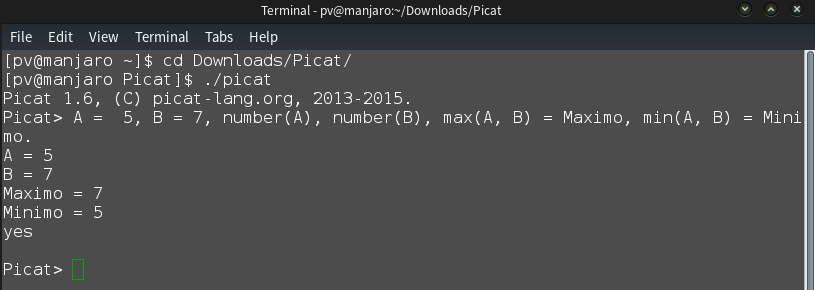
\includegraphics[width=.9\textwidth]{picatnumeros.png}
 \caption{Exemplo de execução}
 %\label{Hiera}
 \end{figure}

\end{frame}

%%%%%%%%%%%%%%%%%%%%%%%%%%%%%%%%%%%%%%%%%%%%%%%%%%%%%%%%%%%%%%%%%%%%%%%%

\subsection{Termo Composto}
\begin{frame}[fragile]   %%%% indica que o ambiente  FRAME é frágil
\frametitle{Termo Composto}
\begin{block}{Descrição}
 Um termo composto se divide entre listas, \textit{strings}, estruturas e outros tipos compostos derivado destes são: vetores, mapas e conjuntos. 
 Entretanto, ambos tem seus elementos acessados via casamento de padrões de fatos, predicados e funções.
\end{block}
\end{frame}

%%%%%%%%%%%%%%%%%%%%%%%%%%%%%%%%%%%%%%%%%%%%%%%%%%%%%%%%%%%%%%%%%%%%%%%%

\subsubsection{Listas}
\begin{frame}[fragile]   %%%% indica que o ambiente  FRAME é frágil
\frametitle{Lista}
\begin{block}{Descrição}
 A forma de uma lista reúne um conjunto de termos e os coloca dentro de colchetes: \texttt{[$t_1,t_2, ... ,t_n$]}.
\end{block}
\end{frame}

%%%%%%%%%%%%%%%%%%%%%%%%%%%%%%%%%%%%%%%%%%%%%%%%%%%%%%%%%%%%%%%%%%%%%%%%

\begin{frame}[fragile]   %%%% indica que o ambiente  FRAME é frágil
\frametitle{Listas}

 \begin{figure}[!ht]
 \centering
 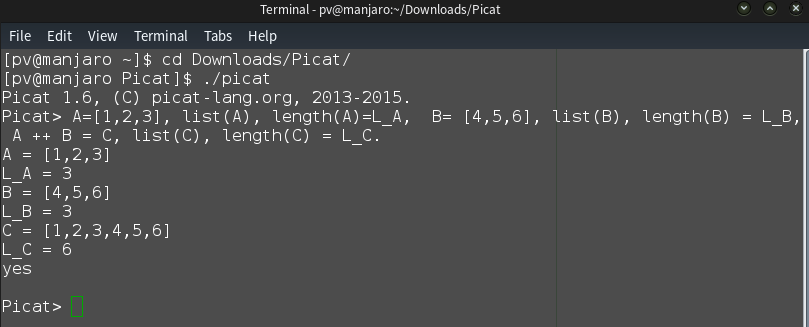
\includegraphics[width=.9\textwidth]{picatlista.png}
 \caption{Exemplo de execução}
 %\label{Hiera}
 \end{figure}

\end{frame}

%%%%%%%%%%%%%%%%%%%%%%%%%%%%%%%%%%%%%%%%%%%%%%%%%%%%%%%%%%%%%%%%%%%%%%%%

\subsubsection{Strings}
\begin{frame}[fragile]   %%%% indica que o ambiente  FRAME é frágil
\frametitle{Strings}
\begin{block}{Descrição}
 Uma \textit{string} pode ser representada em forma de lista, ou seja, cada caractere de uma \textit{string} é um termo de uma lista. 
 Por exemplo: a palavra \texttt{"carro"} pode ser expressa da forma \texttt{[c,a,r,r,o]}..
\end{block}
\end{frame}

%%%%%%%%%%%%%%%%%%%%%%%%%%%%%%%%%%%%%%%%%%%%%%%%%%%%%%%%%%%%%%%%%%%%%%%%

\begin{frame}[fragile]   %%%% indica que o ambiente  FRAME é frágil
\frametitle{Strings}

 \begin{figure}[!ht]
 \centering
 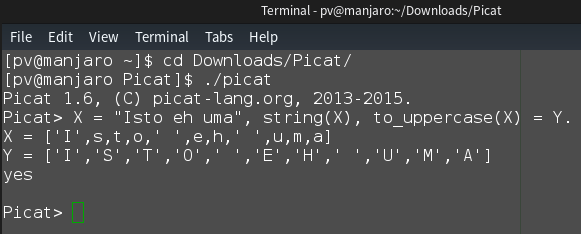
\includegraphics[width=.9\textwidth]{picatstring.png}
 \caption{Exemplo de execução}
 %\label{Hiera}
 \end{figure}

\end{frame}

%%%%%%%%%%%%%%%%%%%%%%%%%%%%%%%%%%%%%%%%%%%%%%%%%%%%%%%%%%%%%%%%%%%%%%%%

\subsubsection{Estruturas}
\begin{frame}[fragile]   %%%% indica que o ambiente  FRAME é frágil
\frametitle{Estruturas}
\begin{block}{Descrição}
  A forma de uma estrutura é definida como \texttt{\$s($t_1$, $t_2$, ...$t_n$)}, 
  onde \texttt{s} é um átomo e \$ é usado para diferenciar uma função. 
  Seus principais elementos são o nome da estrutura que é o átomo que fica na frente e a aridade (número de argumentos do predicado).
\end{block}
\end{frame}

%%%%%%%%%%%%%%%%%%%%%%%%%%%%%%%%%%%%%%%%%%%%%%%%%%%%%%%%%%%%%%%%%%%%%%%%

\begin{frame}[fragile]   %%%% indica que o ambiente  FRAME é frágil
\frametitle{Estruturas}

 \begin{figure}[!ht]
 \centering
 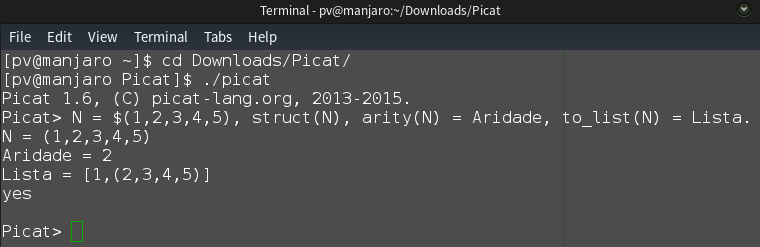
\includegraphics[width=.9\textwidth]{picatestrutura.png}
 \caption{Exemplo de execução}
 %\label{Hiera}
 \end{figure}

\end{frame}

%%%%%%%%%%%%%%%%%%%%%%%%%%%%%%%%%%%%%%%%%%%%%%%%%%%%%%%%%%%%%%%%%%%%%%%%

\subsubsection{Vetores}
\begin{frame}[fragile]   %%%% indica que o ambiente  FRAME é frágil
\frametitle{Vetores}
\begin{block}{Descrição}
  Um vetor ou um \textit{array} tem o formato de $\{t_1, t_2, ... t_n\}$, 
  onde $t_i$ é um termo desta estrutura de aridade  $n$. 
\end{block}
\end{frame}

%%%%%%%%%%%%%%%%%%%%%%%%%%%%%%%%%%%%%%%%%%%%%%%%%%%%%%%%%%%%%%%%%%%%%%%%

\begin{frame}[fragile]   %%%% indica que o ambiente  FRAME é frágil
\frametitle{Vetores}

 \begin{figure}[!ht]
 \centering
 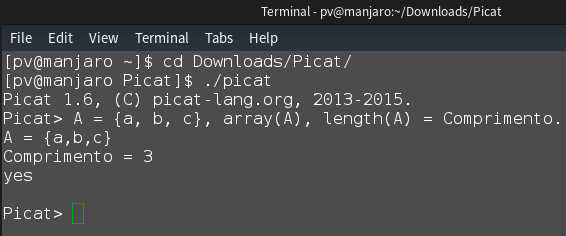
\includegraphics[width=.9\textwidth]{picatvetor.png}
 \caption{Exemplo de execução}
 %\label{Hiera}
 \end{figure}

\end{frame}

%%%%%%%%%%%%%%%%%%%%%%%%%%%%%%%%%%%%%%%%%%%%%%%%%%%%%%%%%%%%%%%%%%%%%%%%

\subsubsection{Mapas}
\begin{frame}[fragile]   %%%% indica que o ambiente  FRAME é frágil
\frametitle{Mapas}
\begin{block}{Descrição}
  Os mapas tem a mesma forma de uma estrutura, porém eles possuem um valor especial para ser usado como chave. 
\end{block}
\end{frame}

%%%%%%%%%%%%%%%%%%%%%%%%%%%%%%%%%%%%%%%%%%%%%%%%%%%%%%%%%%%%%%%%%%%%%%%%

\begin{frame}[fragile]   %%%% indica que o ambiente  FRAME é frágil
\frametitle{Mapas}

 \begin{figure}[!ht]
 \centering
 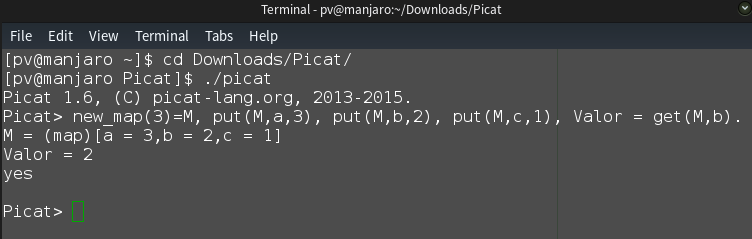
\includegraphics[width=.9\textwidth]{picatmapas.png}
 \caption{Exemplo de execução}
 %\label{Hiera}
 \end{figure}

\end{frame}

%%%%%%%%%%%%%%%%%%%%%%%%%%%%%%%%%%%%%%%%%%%%%%%%%%%%%%%%%%%%%%%%%%%%%%%%

\subsubsection{Conjuntos}
\begin{frame}[fragile]   %%%% indica que o ambiente  FRAME é frágil
\frametitle{Conjuntos}
\begin{block}{Descrição}
  Um conjunto é um mapa onde todos os elementos da estrutura estão associados à uma chave de valor não-numérico. Todas
  as funções existentes para os mapas podem ser também utilizadas.  
  Para criá-lo é necessário o comando \texttt{new\_set}.
\end{block}
\end{frame}

%%%%%%%%%%%%%%%%%%%%%%%%%%%%%%%%%%%%%%%%%%%%%%%%%%%%%%%%%%%%%%%%%%%%%%%%

\begin{frame}[fragile]   %%%% indica que o ambiente  FRAME é frágil
\frametitle{Conjuntos}

 \begin{figure}[!ht]
 \centering
 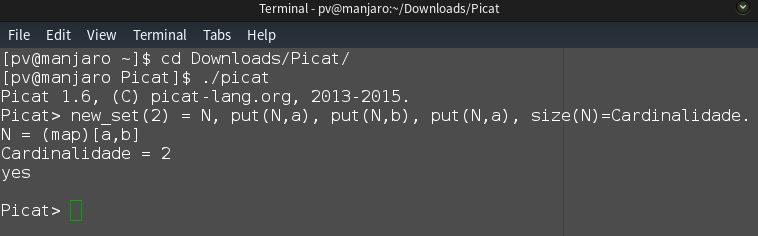
\includegraphics[width=.9\textwidth]{picatconjuntos.png}
 \caption{Exemplo de execução}
 %\label{Hiera}
 \end{figure}

\end{frame}

%%%%%%%%%%%%%%%%%%%%%%%%%%%%%%%%%%%%%%%%%%%%%%%%%%%%%%%%%%%%%%%%%%%%%%%%

\section{Exemplos Práticos}
\begin{frame}[fragile]   %%%% indica que o ambiente  FRAME é frágil
\frametitle{Exemplos Práticos}
\begin{block}{Exemplos podem serem vistos em:}
 \begin{itemize}
  \item \url{https://github.com/claudiosa/CCS/tree/master/picat}
 \end{itemize}

\end{block}

\end{frame}

%%%%%%%%%%%%%%%%%%%%%%%%%%%%%%%%%%%%%%%%%%%%%%%%%%%%%%%%%%%%%%%%%%%%%%%%

\section{Formulário}
\begin{frame}[fragile]
\frametitle{Formulário}

\begin{enumerate}
 \item Qual característica do P.I.C.A.T é mais chamativa?
 %R: multi-paradigma ...(fora objetos), leve  como Python
 \item Em quais aplicações você usaria P.I.C.A.T?
 %R: ensino de uma primeira linguagem 
 \item Quais são os pontos positivos e negativos do P.I.C.A.T que você identifica?
 %R: negativo .... geração de codigo (ainda eh byte-code) e interface com outras linguagens (ainda incipiente)
 \item Se pudesse melhorar algo no P.I.C.A.T, o que melhoraria?
 %R: a interface com outras linguagens 
 \item O P.I.C.A.T pode substituir alguma linguagem?
 %R: Prolog sim ...
 \item Você usaria o P.I.C.A.T no lugar de alguma linguagem como C ou Java?
\end{enumerate}
\end{frame}

\end{document}
